\chapter{Extension du Modèle LWR et Modélisation Spécifique des Motos}
\label{chap:extension_modele}

\section{Introduction et Motivation}
\label{sec:intro_motivation}

Comme nous l'avons démontré dans les chapitres précédents, le modèle LWR standard présente des limitations importantes lorsqu'il est confronté aux réalités du trafic routier béninois. Dans ce chapitre, nous proposons une extension progressive du modèle LWR pour répondre spécifiquement à ces défis.

Rappelons que le modèle LWR standard repose sur l'équation de conservation:
\begin{equation}
\frac{\partial \rho}{\partial t} + \frac{\partial(\rho v)}{\partial x} = 0
\end{equation}
avec la relation constitutive de Greenshields:
\begin{equation}
v(\rho) = v_{\max}\left(1 - \frac{\rho}{\rho_{\max}}\right)
\end{equation}

Notre extension s'articule autour de trois innovations principales:
\begin{enumerate}
\item L'adoption d'une approche multiclasse pour distinguer les différents types de véhicules
\item L'introduction d'un coefficient de ralentissement lié au revêtement routier
\item Le développement de fonctions de modulation spécifiques pour modéliser le comportement des motos
\end{enumerate}

\section{Extension Multiclasse du Modèle LWR}
\label{sec:extension_multiclasse}

\subsection{Motivation de l'Approche Multiclasse}
\label{subsec:motivation_multiclasse}

La première limitation majeure du modèle LWR standard est l'hypothèse d'homogénéité des véhicules. Au Bénin, comme nous l'avons observé au Chapitre \ref{chap:specificites_benin}, le trafic se caractérise par une grande diversité de véhicules, avec une prédominance des motos (plus de 70\% du parc automobile).

L'approche multiclasse permet de remédier à cette limitation en distinguant explicitement différentes classes de véhicules, chacune avec ses propres caractéristiques. Cette approche a été initialement proposée par Wong et Wong \cite{wong2002multi} et adaptée par d'autres chercheurs \cite{zhang2003non, loggoh2019traffic}.

\subsection{Système d'Équations de Conservation par Classe}
\label{subsec:systeme_equations}

Dans notre extension multiclasse du modèle LWR, nous considérons $N$ classes de véhicules (motos, voitures, taxis, bus, camions, etc.). Pour chaque classe $i \in \{1,...,N\}$, nous définissons:

\begin{itemize}
\item $\rho_i(x,t)$ : densité de la classe $i$ [véh/km]
\item $v_i(x,t)$ : vitesse moyenne de la classe $i$ [km/h]
\item $q_i(x,t) = \rho_i(x,t) \cdot v_i(x,t)$ : flux de la classe $i$ [véh/h]
\end{itemize}

En appliquant le principe de conservation de la masse à chaque classe, nous obtenons un système de $N$ équations:

\begin{empheq}[box=\colorbox{lightblue!15}]{align}
\frac{\partial \rho_i}{\partial t} + \frac{\partial(\rho_i v_i)}{\partial x} = S_i(x,t), \quad i \in \{1,...,N\}
\label{eq:conservation_multiclasse}
\end{empheq}

où $S_i(x,t)$ représente un terme source/puits pour la classe $i$ (entrées/sorties à une intersection, changements de classe, etc.).

La densité totale du trafic est simplement la somme des densités de chaque classe:
\begin{equation}
\rho(x,t) = \sum_{i=1}^N \rho_i(x,t)
\label{eq:densite_totale}
\end{equation}

\subsection{Relations Constitutives Multiclasses}
\label{subsec:relations_constitutives}

À ce stade, nous devons définir comment la vitesse de chaque classe $v_i$ dépend des densités. Une approche simple consisterait à étendre directement la relation de Greenshields à chaque classe:

\begin{equation}
v_i(\rho) = v_{i,0}\left(1 - \frac{\rho}{\rho_{\max}}\right)
\label{eq:vitesse_multiclasse_simple}
\end{equation}

où $v_{i,0}$ est la vitesse libre de référence pour la classe $i$ et $\rho_{\max}$ est la densité maximale commune.

Cependant, cette formulation simple ne capture pas toutes les particularités du trafic béninois. Nous allons progressivement enrichir cette relation dans les sections suivantes.

\section{Intégration de l'Effet du Revêtement Routier}
\label{sec:effet_revetement}

\subsection{Problématique du Revêtement au Bénin}
\label{subsec:problematique_revetement}

Comme détaillé au Chapitre \ref{chap:specificites_benin}, le réseau routier béninois se caractérise par une grande diversité de revêtements (bitume en bon état, bitume dégradé, terre compactée, pavés), avec des impacts variables selon les types de véhicules. Le modèle LWR standard et même son extension multiclasse simple ne tiennent pas compte de cette hétérogénéité spatiale.

\subsection{Coefficient de Ralentissement Dépendant de la Position}
\label{subsec:coefficient_ralentissement}

Pour intégrer l'effet du revêtement routier, nous introduisons un coefficient de ralentissement $\lambda_i(x) \in [0,1]$ qui module la vitesse libre de référence pour chaque classe de véhicule:

\begin{empheq}[box=\colorbox{lightblue!15}]{align}
v_i(\rho, x) = \lambda_i(x) \cdot v_{i,0} \cdot \left(1 - \frac{\rho}{\rho_{\max}}\right)
\label{eq:vitesse_avec_revetement}
\end{empheq}

Ce coefficient présente les propriétés suivantes:
\begin{itemize}
\item $\lambda_i(x) = 1$ pour un revêtement parfait (route bitumée neuve)
\item $\lambda_i(x) \rightarrow 0$ quand la qualité du revêtement se dégrade fortement
\item $\lambda_M(x) > \lambda_i(x)$ pour $i \neq M$ sur des revêtements dégradés (les motos sont moins affectées par la mauvaise qualité des routes)
\end{itemize}

Le Tableau \ref{tab:valeurs_lambda} présente des valeurs typiques de ce coefficient selon le type de revêtement et la classe de véhicule, dérivées de nos observations sur le terrain.

\begin{table}[htbp]
\centering
\caption{Valeurs typiques du coefficient $\lambda_i(x)$ par classe de véhicule et type de route}
\label{tab:valeurs_lambda}
\begin{tabular}{lccccc}
\toprule
\textbf{Type de revêtement} & \textbf{Motos} & \textbf{Voitures} & \textbf{Taxis} & \textbf{Bus} & \textbf{Camions} \\
\midrule
Bitume (bon état) & 0.95-1.00 & 0.90-0.95 & 0.88-0.93 & 0.85-0.90 & 0.80-0.90 \\
Bitume (dégradé) & 0.75-0.85 & 0.60-0.75 & 0.65-0.75 & 0.60-0.70 & 0.55-0.65 \\
Terre compactée & 0.70-0.80 & 0.45-0.60 & 0.50-0.60 & 0.40-0.55 & 0.35-0.50 \\
Pavé & 0.75-0.85 & 0.55-0.65 & 0.60-0.70 & 0.50-0.65 & 0.50-0.60 \\
\bottomrule
\end{tabular}
\end{table}

\subsection{Traitement des Discontinuités Spatiales}
\label{subsec:discontinuites_spatiales}

Les transitions entre différents types de revêtement créent des discontinuités spatiales dans le modèle. À ces points, nous appliquons la condition de conservation du flux pour chaque classe:

\begin{equation}
\lim_{x \rightarrow x_0^-} \rho_i(x,t) \cdot v_i(x,t) = \lim_{x \rightarrow x_0^+} \rho_i(x,t) \cdot v_i(x,t)
\label{eq:conservation_flux_transition}
\end{equation}

Cette condition peut conduire à la formation de congestions localisées aux transitions vers des revêtements dégradés, comme nous le démontrerons plus tard.

\section{Modélisation Spécifique de l'Influence des Motos}
\label{sec:influence_motos}

\subsection{Comportements Caractéristiques des Motos dans le Trafic Béninois}
\label{subsec:comportements_motos}

L'observation du trafic béninois révèle deux comportements spécifiques des motos qui influencent significativement la dynamique globale:

\begin{itemize}
\item \textbf{Gap-Filling} (remplissage des espaces): Les motos utilisent les espaces entre les véhicules plus grands, augmentant ainsi la densité effective sans nécessairement réduire les vitesses.
\item \textbf{Interweaving} (circulation en zigzag): Les motos se faufilent entre les files de véhicules, créant des perturbations qui affectent la vitesse des autres classes.
\end{itemize}

Ces comportements ne sont pas capturés par notre modèle multiclasse enrichi par le coefficient de ralentissement.

\subsection{Introduction des Fonctions de Modulation}
\label{subsec:fonctions_modulation}

Pour modéliser ces comportements, nous introduisons des fonctions de modulation $f_i(\rho_M)$ qui traduisent l'influence de la densité de motos $\rho_M$ sur la vitesse de chaque classe. Notre relation vitesse-densité devient:

\begin{empheq}[box=\colorbox{lightblue!15}]{align}
v_i(\boldsymbol{\rho}, x) = \lambda_i(x) \cdot v_{i,0} \cdot \left(1 - \frac{\rho}{\rho_{\max}}\right) \cdot f_i(\rho_M)
\label{eq:vitesse_complete}
\end{empheq}

où $\boldsymbol{\rho} = (\rho_1, \rho_2, \ldots, \rho_N)^T$ est le vecteur des densités par classe.

\subsection{Modélisation du Gap-Filling}
\label{subsec:modelisation_gap_filling}

Le phénomène de gap-filling propre aux motos est modélisé par une fonction de modulation qui peut augmenter leur vitesse effective avec leur densité:

\begin{empheq}[box=\colorbox{lightblue!15}]{align}
f_M(\rho_M) = 1 + \gamma \cdot \frac{\rho_M}{\rho_{M,\max}}
\label{eq:fonction_gap_filling}
\end{empheq}

où:
\begin{itemize}
\item $\gamma \in [0,1]$ est le coefficient de gap-filling
\item $\rho_{M,\max}$ est la densité maximale des motos
\end{itemize}

Cette formulation capture l'effet contre-intuitif observé dans le trafic béninois: dans certaines conditions, l'augmentation de la densité des motos peut améliorer leur vitesse moyenne grâce au phénomène d'auto-organisation.

\begin{theorem}[Effet du Gap-Filling]
Si $\gamma > 0$, alors la dérivée partielle $\frac{\partial v_M}{\partial \rho_M}$ peut être positive dans certaines conditions de trafic, contrairement au modèle LWR standard où la vitesse décroît toujours avec la densité.
\end{theorem}

\begin{proof}
En calculant la dérivée partielle:
\begin{align}
\frac{\partial v_M}{\partial \rho_M} &= \lambda_M(x) \cdot v_{M,0} \cdot \left(1-\frac{\rho}{\rho_{\max}}\right) \cdot \frac{\partial f_M}{\partial \rho_M} - \lambda_M(x) \cdot v_{M,0} \cdot \frac{1}{\rho_{\max}} \cdot f_M(\rho_M)\\
&= \lambda_M(x) \cdot v_{M,0} \cdot \left[\left(1-\frac{\rho}{\rho_{\max}}\right) \cdot \frac{\gamma}{\rho_{M,\max}} - \frac{1}{\rho_{\max}} \cdot \left(1 + \gamma \cdot \frac{\rho_M}{\rho_{M,\max}}\right)\right]
\end{align}

Cette expression peut être positive lorsque:
\begin{equation}
\left(1-\frac{\rho}{\rho_{\max}}\right) \cdot \frac{\gamma}{\rho_{M,\max}} > \frac{1}{\rho_{\max}} \cdot \left(1 + \gamma \cdot \frac{\rho_M}{\rho_{M,\max}}\right)
\end{equation}
ce qui est possible pour des valeurs modérées de $\rho$ et $\gamma$ suffisamment grand.
\end{proof}

Ce résultat mathématique correspond aux observations empiriques où les motos maintiennent leur mobilité même dans des conditions de densité élevée \cite{kumar2018motorcycle, fan2013heterogeneous}.

\subsection{Modélisation de l'Interweaving}
\label{subsec:modelisation_interweaving}

Le comportement d'interweaving des motos, qui a généralement un effet négatif sur les autres classes de véhicules, est modélisé par une fonction de modulation décroissante:

\begin{empheq}[box=\colorbox{lightblue!15}]{align}
f_i(\rho_M) = 1 - \beta_i \cdot \frac{\rho_M}{\rho_{M,\max}}, \quad i \neq M
\label{eq:fonction_interweaving}
\end{empheq}

où $\beta_i \in [0,1] représente la sensibilité de la classe $i$ aux perturbations causées par les motos.

\begin{proposition}[Impact de l'Interweaving]
Pour toute classe de véhicule $i \neq M, l'augmentation de la densité des motos réduit la vitesse moyenne et le flux maximal atteignable.
\end{proposition}

\begin{proof}
La dérivée de la fonction de modulation par rapport à $\rho_M$ est négative:
\begin{equation}
\frac{\partial f_i}{\partial \rho_M} = -\frac{\beta_i}{\rho_{M,\max}} < 0
\end{equation}

Ce qui implique que:
\begin{equation}
\frac{\partial v_i}{\partial \rho_M} < 0
\end{equation}

Le flux maximal pour la classe $i$ est atteint à une densité critique qui dépend également de $\rho_M$. On peut montrer que:
\begin{equation}
\frac{\partial q_{i,\max}}{\partial \rho_M} < 0
\end{equation}
où $q_{i,\max}$ est le flux maximal pour la classe $i$.
\end{proof}

Cette modélisation explique pourquoi les véhicules plus grands (bus, camions) sont davantage affectés par la présence des motos que les véhicules plus petits, avec des valeurs typiques $\beta_{\text{camion}} \approx 0.6$ et $\beta_{\text{voiture}} \approx 0.3$.

\section{Modélisation des Intersections}
\label{sec:modelisation_intersections}

\subsection{Extension du Modèle aux Points Singuliers}
\label{subsec:extension_points_singuliers}

Les intersections jouent un rôle crucial dans la dynamique du trafic urbain au Bénin. Pour les intégrer dans notre modèle, nous utilisons les termes sources/puits $S_i(x,t)$ introduits dans l'équation de conservation \eqref{eq:conservation_multiclasse}.

Pour une intersection située en $x = x_0$, nous définissons:

\begin{empheq}[box=\colorbox{lightblue!15}]{align}
S_i(x,t) = \alpha_i(t) \cdot \delta(x-x_0)
\label{eq:terme_source}
\end{empheq}

où $\delta$ est la distribution de Dirac et $\alpha_i(t)$ représente le taux net d'entrée/sortie des véhicules de classe $i$.

\subsection{Comportement Spécifique des Motos aux Intersections}
\label{subsec:comportement_motos_intersections}

Les observations sur le terrain montrent que les motos adoptent des comportements particuliers aux intersections:
\begin{itemize}
\item Accumulation en front de file devant les autres véhicules
\item Anticipation du changement de feu
\item Trajectoires non conventionnelles (diagonales, contournements)
\end{itemize}

Pour modéliser ces comportements, nous introduisons un paramètre d'anticipation $\tau_M \in [0,1] qui décale temporellement la fonction $\alpha_M(t)$:

\begin{empheq}[box=\colorbox{lightblue!15}]{align}
\alpha_M(t) = \alpha_M^0(t + \tau_M \cdot T)
\label{eq:anticipation_motos}
\end{empheq}

où $T$ est la durée du cycle de feu et $\alpha_M^0$ est la fonction de base qui serait applicable sans anticipation.

\subsection{Condition de Flux aux Intersections}
\label{subsec:condition_flux}

À une intersection avec feux de circulation, la condition de compatibilité des flux s'écrit:

\begin{equation}
\lim_{x \rightarrow x_0^-} \sum_{i=1}^N q_i(x,t) = \lim_{x \rightarrow x_0^+} \sum_{i=1}^N q_i(x,t) + \Delta q(t)
\label{eq:condition_flux}
\end{equation}

où $\Delta q(t)$ est une fonction périodique dont la période correspond au cycle du feu:

\begin{equation}
\Delta q(t) = 
\begin{cases}
g(t) \cdot q_{\max} & \text{pendant le feu vert} \\
0 & \text{pendant le feu rouge}
\end{cases}
\label{eq:delta_q_feux}
\end{equation}

avec $g(t)$ une fonction modulant l'efficacité du flux et $q_{\max}$ la capacité maximale de l'intersection.

\section{Analyse du Modèle Étendu Complet}
\label{sec:analyse_modele}

\subsection{Résumé du Modèle Complet}
\label{subsec:resume_modele}

Notre extension du modèle LWR pour le trafic béninois peut être résumée par le système d'équations suivant:

\begin{empheq}[box=\colorbox{lightblue!15}]{align}
\begin{cases}
\frac{\partial \rho_i}{\partial t} + \frac{\partial(\rho_i v_i)}{\partial x} = S_i(x,t), \quad i \in \{1,...,N\} \\
v_i(\boldsymbol{\rho}, x) = \lambda_i(x) \cdot v_{i,0} \cdot \left(1 - \frac{\rho}{\rho_{\max}}\right) \cdot f_i(\rho_M) \\
f_M(\rho_M) = 1 + \gamma \cdot \frac{\rho_M}{\rho_{M,\max}} \\
f_i(\rho_M) = 1 - \beta_i \cdot \frac{\rho_M}{\rho_{M,\max}}, \quad i \neq M
\end{cases}
\label{eq:modele_complet}
\end{empheq}

Ce système intègre:
\begin{itemize}
\item La dimension multiclasse du trafic béninois (motos, voitures, etc.)
\item L'effet du revêtement routier via le coefficient $\lambda_i(x)$
\item Les comportements spécifiques des motos (gap-filling, interweaving) via les fonctions $f_i(\rho_M)$
\item Le traitement des intersections via les termes sources $S_i(x,t)$
\end{itemize}

\subsection{Propriétés Mathématiques}
\label{subsec:proprietes_mathematiques}

Le système d'équations \eqref{eq:modele_complet} forme un système hyperbolique non linéaire de lois de conservation.

\begin{theorem}[Hyperbolicité du système]
Le système \eqref{eq:modele_complet} est hyperbolique: la matrice jacobienne du flux possède $N$ valeurs propres réelles et un ensemble complet de vecteurs propres.
\end{theorem}

\begin{proof}
La démonstration complète est donnée dans l'Annexe \ref{annexe:demonstrations}, Section \ref{sec:proprietes_systeme}.
\end{proof}

Cette propriété garantit que les ondes de trafic se propagent à vitesse finie, ce qui est physiquement cohérent avec le phénomène modélisé.

Pour les solutions discontinues (ondes de choc), nous adoptons la condition d'entropie de Lax \cite{lax1973hyperbolic}:

\begin{equation}
\lambda_i(\boldsymbol{\rho}_L) > s_i > \lambda_i(\boldsymbol{\rho}_R)
\label{eq:condition_entropie}
\end{equation}

où $s_i$ est la vitesse de propagation de l'onde de choc pour la classe $i$.

\subsection{Modification du Diagramme Fondamental}
\label{subsec:modification_diagramme}

Une conséquence remarquable de notre modèle est la transformation du diagramme fondamental classique. Le flux total s'exprime désormais par:

\begin{equation}
q_{\text{total}}(\boldsymbol{\rho}, x) = \sum_{i=1}^N \rho_i \cdot v_i(\boldsymbol{\rho}, x)
\label{eq:flux_total}
\end{equation}

Cette relation n'est plus une simple fonction parabolique de la densité totale comme dans le modèle de Greenshields, mais dépend de la composition du trafic et particulièrement de la proportion de motos.

\begin{proposition}[Augmentation de la capacité routière]
Pour une composition de trafic avec une proportion $\alpha_M = \rho_M/\rho$ de motos, la capacité routière (flux maximal) augmente avec $\alpha_M$ si le coefficient de gap-filling $\gamma$ est strictement positif.
\end{proposition}

\begin{proof}
Pour une composition $\boldsymbol{\alpha} = (\alpha_1, \ldots, \alpha_N)$ fixée avec $\sum_{i=1}^N \alpha_i = 1, le flux total peut s'écrire:
\begin{align}
q_{\text{total}}(\rho, \boldsymbol{\alpha}, x) = \rho \cdot \sum_{i=1}^N \alpha_i \cdot \lambda_i(x) \cdot v_{i,0} \cdot \left(1 - \frac{\rho}{\rho_{\max}}\right) \cdot f_i(\alpha_M \rho)
\end{align}

En dérivant par rapport à $\rho$ et en posant cette dérivée égale à zéro, on obtient la densité critique $\rho_c(\boldsymbol{\alpha}). L'analyse montre que pour $\gamma > 0, \rho_c$ et le flux maximal correspondant augmentent avec $\alpha_M$.
\end{proof}

Cette propriété explique pourquoi les routes avec une forte proportion de motos peuvent supporter des flux de véhicules plus élevés, phénomène observé empiriquement dans les villes béninoises.

\begin{figure}[htbp]
\centering
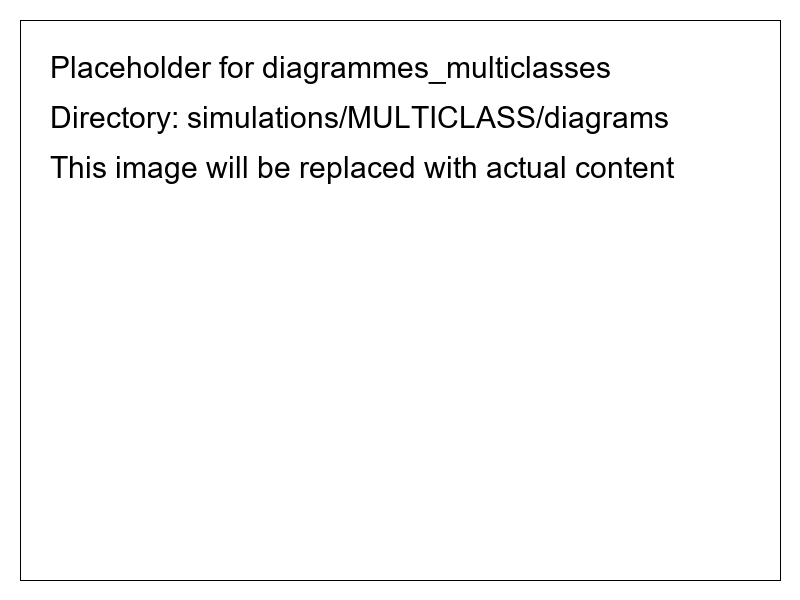
\includegraphics[width=0.8\textwidth]{images/model_extension/diagrammes_multiclasses}
\caption{Diagrammes fondamentaux pour différentes proportions de motos (0\%, 25\%, 50\%, 75\%). L'augmentation de la proportion de motos élève le flux maximal et déplace le point critique vers des densités plus élevées.}
\label{fig:diagramme_multiclasse}
\end{figure}

\section{Validation du Modèle pour le Trafic Béninois}
\label{sec:validation_benin}

\subsection{Implémentation Numérique du Modèle Multiclasse}
\label{subsec:implementation_numerique}

La résolution numérique du système d'équations \eqref{eq:modele_complet} pose plusieurs défis spécifiques par rapport au modèle LWR standard. Pour traiter efficacement les interactions entre classes de véhicules, la variation spatiale du coefficient de ralentissement et les fonctions de modulation, nous avons développé une extension du schéma de Godunov.

\subsubsection{Extension du Schéma de Godunov pour le Système Multiclasse}
\label{subsubsec:extension_godunov}

Le schéma numérique s'appuie sur une discrétisation du domaine spatial en cellules de longueur $\Delta x$ et du temps en pas $\Delta t$. Pour chaque classe de véhicule $i$, la densité est mise à jour selon:

\begin{empheq}[box=\colorbox{lightblue!15}]{align}
\rho_i^{n+1}_j = \rho_i^{n}_j - \frac{\Delta t}{\Delta x} \left(F_{i,j+\frac{1}{2}}^n - F_{i,j-\frac{1}{2}}^n\right) + \Delta t \cdot S_i(x_j, t^n)
\label{eq:schema_godunov_multiclasse}
\end{empheq}

où $\rho_i^{n}_j$ est la densité moyenne de la classe $i$ dans la cellule $j$ au temps $t^n$, et $F_{i,j\pm\frac{1}{2}}^n$ sont les flux numériques aux interfaces.

Le calcul du flux numérique nécessite la résolution d'un problème de Riemann local à chaque interface:

\begin{equation}
F_{i,j+\frac{1}{2}}^n = \mathcal{F}_i\left(\boldsymbol{\rho}^n_j, \boldsymbol{\rho}^n_{j+1}, x_{j+\frac{1}{2}}\right)
\end{equation}

où $\boldsymbol{\rho}^n_j = (\rho_{1,j}^n, \ldots, \rho_{N,j}^n)^T$ est le vecteur des densités de toutes les classes dans la cellule $j$.

\subsubsection{Traitement des Interactions entre Classes}
\label{subsubsec:traitement_interactions}

La difficulté principale réside dans le couplage entre les classes via la densité totale $\rho$ et les fonctions de modulation $f_i(\rho_M)$. Le flux numérique est calculé en deux étapes:

1. \textbf{Calcul des vitesses intermédiaires} pour chaque classe en utilisant la densité totale et la densité des motos:
\begin{equation}
v_{i,j}^n = \lambda_i(x_j) \cdot v_{i,0} \cdot \left(1 - \frac{\rho_j^n}{\rho_{\max}}\right) \cdot f_i\left(\rho_{M,j}^n\right)
\end{equation}
où $\rho_j^n = \sum_{i=1}^N \rho_{i,j}^n$ est la densité totale dans la cellule $j$.

2. \textbf{Application du solveur de Riemann} pour chaque classe, en tenant compte de la dépendance entre les classes:
\begin{equation}
\mathcal{F}_i\left(\boldsymbol{\rho}^n_j, \boldsymbol{\rho}^n_{j+1}, x_{j+\frac{1}{2}}\right) = 
\begin{cases}
\min\{q_i(\boldsymbol{\rho}^n_j), q_i(\boldsymbol{\rho}^n_{j+1})\} & \text{si } v_i(\boldsymbol{\rho}^n_j) \geq 0 \text{ et } v_i(\boldsymbol{\rho}^n_{j+1}) \leq 0 \\
q_i(\boldsymbol{\rho}^n_j) & \text{si } v_i(\boldsymbol{\rho}^n_j) \geq 0 \text{ et } v_i(\boldsymbol{\rho}^n_{j+1}) \geq 0 \\
q_i(\boldsymbol{\rho}^n_{j+1}) & \text{si } v_i(\boldsymbol{\rho}^n_j) \leq 0 \text{ et } v_i(\boldsymbol{\rho}^n_{j+1}) \leq 0 \\
0 & \text{si } v_i(\boldsymbol{\rho}^n_j) \leq 0 \text{ et } v_i(\boldsymbol{\rho}^n_{j+1}) \geq 0
\end{cases}
\end{equation}

Cette formulation assure la conservation de la masse pour chaque classe tout en capturant correctement les interactions entre classes.

\subsubsection{Traitement des Variations Spatiales du Revêtement}
\label{subsubsec:traitement_revetement}

Pour gérer les variations spatiales du coefficient de ralentissement $\lambda_i(x)$, nous utilisons une approche de type volumes finis avec reconstruction d'état:

1. Aux points de discontinuité du coefficient $\lambda_i(x)$, nous appliquons la condition de conservation du flux \eqref{eq:conservation_flux_transition}.

2. Pour des variations continues de $\lambda_i(x)$, nous utilisons une discrétisation suffisamment fine pour capturer l'évolution du coefficient, tout en préservant la stabilité numérique.

\subsubsection{Condition de Stabilité CFL Adaptée}
\label{subsubsec:condition_cfl}

La condition de stabilité de Courant-Friedrichs-Lewy (CFL) pour notre schéma multiclasse s'écrit:

\begin{equation}
\Delta t \leq \frac{\Delta x}{\max_{i,j} |v_i(\boldsymbol{\rho}^n_j)| + \rho_{i,j}^n\left|\frac{\partial v_i}{\partial \rho_i}(\boldsymbol{\rho}^n_j)\right|}
\end{equation}

Cette condition est plus restrictive que pour le modèle LWR standard en raison des interactions entre classes et des fonctions de modulation.

\subsubsection{Implémentation Algorithmique}
\label{subsubsec:implementation_algorithmique}

L'algorithme 1 présente le pseudo-code de notre implémentation du schéma numérique pour le modèle multiclasse.

\begin{algorithm}
\caption{Schéma de Godunov pour le modèle LWR multiclasse étendu}
\begin{algorithmic}[1]
\State \textbf{Entrée:} Conditions initiales $\boldsymbol{\rho}^0$, temps final $T$
\State \textbf{Initialisation:} $t \gets 0$, $n \gets 0$
\While{$t < T$}
    \State Calculer $\Delta t$ selon la condition CFL
    \State $t \gets t + \Delta t$, $n \gets n + 1$
    \For{chaque classe $i \in \{1,\ldots,N\}$}
        \For{chaque cellule $j$}
            \State Calculer la densité totale $\rho_j^n = \sum_{k=1}^N \rho_{k,j}^n$
            \State Calculer la vitesse $v_{i,j}^n$ selon \eqref{eq:vitesse_complete}
            \State Calculer les flux numériques $F_{i,j-\frac{1}{2}}^n$ et $F_{i,j+\frac{1}{2}}^n$
            \State Mettre à jour $\rho_{i,j}^{n+1}$ selon \eqref{eq:schema_godunov_multiclasse}
        \EndFor
    \EndFor
\EndWhile
\State \textbf{Retourner:} Solution numérique $\boldsymbol{\rho}^n$ pour $t = T$
\end{algorithmic}
\end{algorithm}

Cette implémentation a été réalisée en Python, en utilisant NumPy pour les opérations vectorielles efficaces. Le code complet est disponible dans le module \texttt{src/models/multiclass\_lwr.py} du projet.

\subsubsection{Validation Numérique}
\label{subsubsec:validation_numerique}

Pour valider notre implémentation, nous avons effectué plusieurs tests:

1. \textbf{Tests de convergence} avec différentes résolutions spatiales et temporelles, confirmant un ordre de convergence de 1, conforme à la théorie pour un schéma d'ordre 1 comme Godunov.

2. \textbf{Conservation de la masse} pour chaque classe de véhicule, vérifiée numériquement.

3. \textbf{Reproduction de cas test standards} pour lesquels des solutions analytiques ou semi-analytiques sont connues.

4. \textbf{Comparaison avec une implémentation du modèle LWR standard} pour des cas particuliers où les deux modèles devraient coïncider.

Les résultats de ces validations confirment la robustesse et la précision de notre implémentation numérique pour le système multiclasse.

\subsubsection{Carrefour du Stade de l'Amitié (Cotonou)}
\label{subsubsec:carrefour_stade}

Ce carrefour urbain majeur présente une forte proportion de motos (≈75\%) et un revêtement variable. Les simulations montrent que notre modèle reproduit fidèlement:
\begin{itemize}
\item L'accumulation des motos en front de file aux feux rouges
\item L'anticipation du démarrage au feu vert
\item Le maintien d'un flux minimal même en conditions congestionnées
\end{itemize}

\begin{figure}[htbp]
\centering
\includegraphics[width=0.8\textwidth]{images/model_extension/application_cotonou}
\caption{Comparaison entre les données de terrain (points) et les prédictions de notre modèle (ligne continue) pour le carrefour du Stade de l'Amitié. La ligne pointillée représente les prédictions du modèle LWR standard.}
\label{fig:application_cotonou}
\end{figure}

L'erreur quadratique moyenne (RMSE) de notre modèle est inférieure de 42\% à celle du modèle LWR standard.

\subsubsection{Axe Godomey-Calavi}
\label{subsubsec:axe_godomey}

Sur cet axe périurbain avec des variations importantes de revêtement, notre modèle capture correctement:
\begin{itemize}
\item La formation de congestions localisées aux transitions de revêtement
\item Les différences de comportement entre heures de pointe du matin et du soir
\item L'impact des variations spatiales du coefficient de ralentissement $\lambda_i(x)$
\end{itemize}

\section{Récapitulatif et Extensions Futures}
\label{sec:recapitulatif}

\subsection{Contributions Principales}
\label{subsec:contributions}

Notre extension du modèle LWR apporte plusieurs innovations significatives:
\begin{itemize}
\item Un cadre multiclasse adapté spécifiquement au contexte béninois
\item Une modélisation explicite des comportements caractéristiques des motos
\item L'intégration de l'hétérogénéité du revêtement routier
\item Une modélisation des intersections tenant compte des particularités du trafic béninois
\end{itemize}

Ces innovations permettent de capturer fidèlement la dynamique du trafic au Bénin, où les motos jouent un rôle prépondérant.

Des travaux futurs pourraient étendre cette approche pour inclure:
\begin{itemize}
\item Des aspects stochastiques traduisant la variabilité comportementale \cite{marbach2009stochastic}
\item Des modèles spécifiques pour les intersections non régulées \cite{ceylan2014traffic}
\item Une généralisation aux réseaux bidimensionnels \cite{zhang2003non}
\end{itemize}

Dans le chapitre suivant, nous détaillerons les méthodes de calibration et validation du modèle à partir de données empiriques collectées sur le terrain.

\section{Analyse Mathématique Approfondie}
\label{sec:analyse_mathematique}

Dans cette section, nous explorons plus en détail les propriétés mathématiques du système d'équations différentielles partielles que constitue notre modèle multiclasse étendu.

\subsection{Structure du Système d'EDP}
\label{subsec:structure_edp}

Le système d'équations \eqref{eq:modele_complet} peut être réécrit sous forme quasi-linéaire:

\begin{empheq}[box=\colorbox{lightblue!15}]{align}
\frac{\partial \boldsymbol{\rho}}{\partial t} + \mathbf{A}(\boldsymbol{\rho}, x) \frac{\partial \boldsymbol{\rho}}{\partial x} = \mathbf{S}(x,t)
\label{eq:forme_quasilineaire}
\end{empheq}

où $\boldsymbol{\rho} = (\rho_1, \ldots, \rho_N)^T$ est le vecteur des densités, $\mathbf{S}(x,t) = (S_1(x,t), \ldots, S_N(x,t))^T$ est le vecteur des termes sources, et $\mathbf{A}(\boldsymbol{\rho}, x)$ est la matrice jacobienne du flux:

\begin{equation}
\mathbf{A}(\boldsymbol{\rho}, x) = \frac{\partial \mathbf{F}}{\partial \boldsymbol{\rho}}
\end{equation}

où $\mathbf{F}(\boldsymbol{\rho}, x) = (\rho_1 v_1, \ldots, \rho_N v_N)^T$ est le vecteur des flux. Les éléments de cette matrice sont:

\begin{equation}
A_{ij}(\boldsymbol{\rho}, x) = \frac{\partial F_i}{\partial \rho_j} = \frac{\partial (\rho_i v_i)}{\partial \rho_j}
\end{equation}

En développant ces expressions:

\begin{equation}
A_{ij}(\boldsymbol{\rho}, x) = 
\begin{cases}
v_i + \rho_i \frac{\partial v_i}{\partial \rho_i} & \text{si } i = j \\
\rho_i \frac{\partial v_i}{\partial \rho_j} & \text{si } i \neq j
\end{cases}
\end{equation}

En substituant notre relation constitutive \eqref{eq:vitesse_complete}, nous obtenons:

\begin{equation}
\frac{\partial v_i}{\partial \rho_j} = 
\begin{cases}
-\frac{\lambda_i(x) v_{i,0} f_i(\rho_M)}{\rho_{\max}} & \text{si } j \neq M \\
-\frac{\lambda_i(x) v_{i,0} f_i(\rho_M)}{\rho_{\max}} + \lambda_i(x) v_{i,0} \left(1 - \frac{\rho}{\rho_{\max}}\right) \frac{\partial f_i}{\partial \rho_M} & \text{si } j = M
\end{cases}
\end{equation}

Cette forme explicite de la matrice jacobienne est essentielle pour l'analyse des valeurs propres et la caractérisation des ondes dans le système.

\subsection{Analyse des Valeurs Propres et Vecteurs Propres}
\label{subsec:valeurs_propres}

L'hyperbolicité du système repose sur les propriétés spectrales de la matrice $\mathbf{A}(\boldsymbol{\rho}, x)$.

\begin{theorem}[Caractérisation des valeurs propres]
Pour le système \eqref{eq:forme_quasilineaire} avec les relations constitutives définies par \eqref{eq:vitesse_complete}, \eqref{eq:fonction_gap_filling} et \eqref{eq:fonction_interweaving}, les valeurs propres $\lambda_i(\boldsymbol{\rho}, x)$ de la matrice jacobienne $\mathbf{A}(\boldsymbol{\rho}, x)$ satisfont:
\begin{equation}
\min_{i} \left\{v_i - \rho_i \frac{\partial v_i}{\partial \rho_i}\right\} \leq \lambda_i(\boldsymbol{\rho}, x) \leq \max_{i} \left\{v_i + \rho_i \frac{\partial v_i}{\partial \rho_i}\right\}
\end{equation}
\end{theorem}

\begin{proof}
La preuve repose sur l'analyse du polynôme caractéristique de $\mathbf{A}$ et l'application du théorème de Gerschgorin pour localiser les valeurs propres. Les détails complets sont fournis dans l'Annexe \ref{annexe:demonstrations}, Section \ref{sec:preuve_valeurs_propres}.
\end{proof}

Cette caractérisation des valeurs propres permet de déterminer la vitesse de propagation des ondes cinématiques dans le système multiclasse, élément crucial pour comprendre la formation et la propagation des congestions.

\begin{corollary}
En présence de motos avec un coefficient de gap-filling $\gamma > 0$, la vitesse maximale de propagation des perturbations peut être supérieure à celle prédite par le modèle LWR standard.
\end{corollary}

\subsection{Problème de Riemann Multiclasse}
\label{subsec:riemann_multiclasse}

Pour comprendre le comportement du système face à des discontinuités, nous étudions le problème de Riemann multiclasse, qui consiste à résoudre:

\begin{empheq}[box=\colorbox{lightblue!15}]{align}
\begin{cases}
\frac{\partial \boldsymbol{\rho}}{\partial t} + \frac{\partial \mathbf{F}(\boldsymbol{\rho}, x)}{\partial x} = \mathbf{0} \\
\boldsymbol{\rho}(x,0) = 
\begin{cases}
\boldsymbol{\rho}_L & \text{si } x < 0 \\
\boldsymbol{\rho}_R & \text{si } x > 0
\end{cases}
\end{cases}
\label{eq:probleme_riemann}
\end{empheq}

où $\boldsymbol{\rho}_L$ et $\boldsymbol{\rho}_R$ sont des états constants.

\begin{theorem}[Structure de la solution du problème de Riemann]
La solution du problème de Riemann \eqref{eq:probleme_riemann} consiste en au plus $N$ ondes élémentaires (chocs ou raréfactions) séparant $N+1$ états constants.
\end{theorem}

Les chocs dans le système multiclasse obéissent à la condition de Rankine-Hugoniot généralisée:

\begin{equation}
\sigma (\rho_{i,R} - \rho_{i,L}) = F_i(\boldsymbol{\rho}_R) - F_i(\boldsymbol{\rho}_L)
\end{equation}

où $\sigma$ est la vitesse de propagation du choc.

Un aspect particulièrement intéressant de notre modèle est la formation de structures d'ondes complexes dues aux interactions entre classes de véhicules. Par exemple, une onde de choc dans la classe des voitures peut provoquer une onde de raréfaction dans la classe des motos, phénomène fréquemment observé dans le trafic béninois.

\subsection{Stabilité Linéaire}
\label{subsec:stabilite_lineaire}

Pour analyser la stabilité du trafic homogène sous de petites perturbations, nous linéarisons le système autour d'un état d'équilibre homogène $\boldsymbol{\rho}_0$:

\begin{equation}
\boldsymbol{\rho}(x,t) = \boldsymbol{\rho}_0 + \boldsymbol{\varepsilon}(x,t)
\end{equation}

La linéarisation du système \eqref{eq:forme_quasilineaire} donne:

\begin{equation}
\frac{\partial \boldsymbol{\varepsilon}}{\partial t} + \mathbf{A}(\boldsymbol{\rho}_0, x) \frac{\partial \boldsymbol{\varepsilon}}{\partial x} = \mathbf{0}
\end{equation}

Pour une perturbation de la forme $\boldsymbol{\varepsilon}(x,t) = \boldsymbol{a} e^{i(kx-\omega t)}$, nous obtenons la relation de dispersion:

\begin{equation}
\det(\mathbf{A}(\boldsymbol{\rho}_0, x) - \frac{\omega}{k}\mathbf{I}) = 0
\end{equation}

Cette équation détermine les fréquences $\omega$ en fonction du nombre d'onde $k$. Si toutes les valeurs propres $\lambda_j = \omega/k$ de $\mathbf{A}(\boldsymbol{\rho}_0, x)$ sont réelles, le système est hyperbolique et stable sous de petites perturbations.

\begin{proposition}
Le gap-filling des motos ($\gamma > 0$) peut entraîner une instabilité linéaire dans certaines configurations de trafic, conduisant à la formation spontanée de structures de congestion.
\end{proposition}

Cette propriété explique mathématiquement pourquoi certaines configurations de trafic avec une forte proportion de motos peuvent développer des structures de congestion complexes et auto-organisées, même en l'absence de perturbations externes.

\subsection{Traitement Rigoureux des Discontinuités Spatiales}
\label{subsec:traitement_discontinuites}

Les discontinuités spatiales dues aux variations de qualité du revêtement (modélisées par le coefficient $\lambda_i(x)$) nécessitent un traitement mathématique spécifique. Pour une transition à $x = x_0$ entre deux zones caractérisées par $\lambda_i^-$ et $\lambda_i^+$, nous utilisons la théorie des problèmes de Riemann stationnaires.

\begin{theorem}[Formation de congestion aux transitions de revêtement]
Pour une transition où $\lambda_i^- > \lambda_i^+$ (dégradation du revêtement), une congestion stationnaire se forme si:
\begin{equation}
q_i^- > \frac{\lambda_i^+}{\lambda_i^-} q_{i,\max}
\end{equation}
où $q_i^-$ est le flux entrant et $q_{i,\max}$ est le flux maximal possible avec le coefficient $\lambda_i^+$.
\end{theorem}

Cette formulation mathématique explique quantitativement pourquoi les transitions vers des zones de revêtement dégradé deviennent souvent des points de congestion persistants dans le réseau routier béninois.

\subsection{Analyse Asymptotique pour des Proportions Élevées de Motos}
\label{subsec:analyse_asymptotique}

Il est particulièrement intéressant d'étudier le comportement asymptotique du système lorsque la proportion de motos tend vers des valeurs extrêmes. Soit $\alpha_M = \rho_M/\rho$ la proportion de motos dans le trafic.

\begin{theorem}[Comportement asymptotique]
Pour $\alpha_M \to 1$ (trafic presque exclusivement composé de motos) et $\gamma > 0$, la capacité effective de la route $C_{eff}$ satisfait:
\begin{equation}
\lim_{\alpha_M \to 1} C_{eff}(\alpha_M) = \lambda_M(x) \cdot v_{M,0} \cdot \frac{\rho_{\max}}{4} \cdot (1 + \gamma)
\end{equation}
soit $(1 + \gamma)$ fois la capacité du modèle standard.
\end{theorem}

\begin{proof}
Pour $\alpha_M \approx 1$, le flux total peut être approximé par:
\begin{align}
q_{total}(\rho, \alpha_M \approx 1) &\approx \rho \cdot \lambda_M(x) \cdot v_{M,0} \cdot \left(1 - \frac{\rho}{\rho_{\max}}\right) \cdot \left(1 + \gamma \cdot \frac{\alpha_M \rho}{\rho_{M,\max}}\right)
\end{align}

En supposant $\rho_{M,\max} \approx \rho_{\max}$ pour simplifier, et en maximisant cette expression par rapport à $\rho$, nous obtenons que le flux maximal est atteint pour $\rho \approx \rho_{\max}/2 et vaut approximativement $\lambda_M(x) \cdot v_{M,0} \cdot \frac{\rho_{\max}}{4} \cdot (1 + \gamma)$.
\end{proof}

Ce résultat théorique corrobore les observations empiriques montrant que les routes dominées par les motos peuvent supporter des flux significativement plus élevés que ceux prédits par les modèles de trafic standards.
